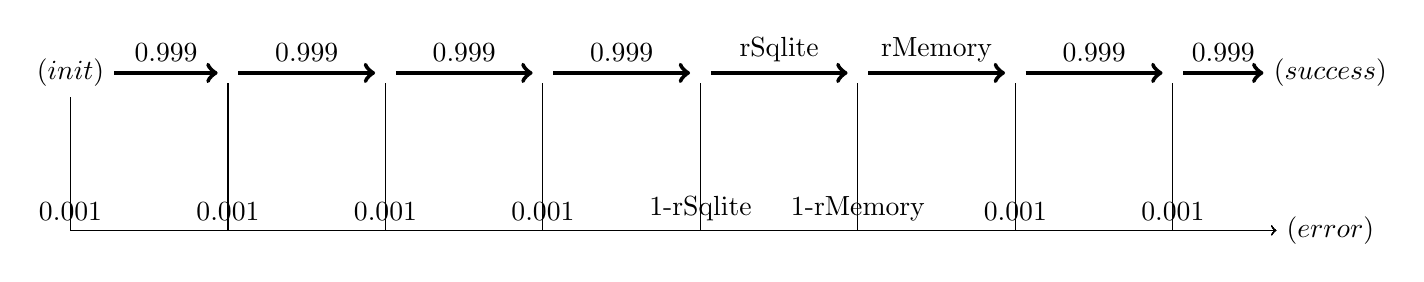
\begin{tikzpicture}[thick]
%\draw[help lines, step=1cm] (0,0) grid +(10,15);
%%%%%%%%%%%%%%%%%%%%%%%%%%%%%%% FDTMC for Oxygenation / Temperature
\node(init) at (0,7){$(init)$};
\node(s1) at (2,7){};
\node(s2) at (4,7){};
\node(s3) at (6,7){};
\node(s4) at (8,7){};
\node(s5) at (10,7){};
\node(s6) at (12,7){};
\node(s7) at (14,7){};
\node(success) at (16,7){$(success)$};
\node(error) at (16,5){$(error)$};
\draw[->, ultra thick] (init) -- node[draw=none, above]{0.999}(s1);
\draw[->, ultra thick] (s1) -- node[draw=none, above]{0.999}(s2);
\draw[->, ultra thick] (s2) -- node[draw=none, above]{0.999}(s3);
\draw[->, ultra thick] (s3) -- node[draw=none, above]{0.999}(s4);
\draw[->, ultra thick] (s4) -- node[draw=none, above]{rSqlite}(s5);
\draw[->, ultra thick] (s5) -- node[draw=none, above]{rMemory}(s6);
\draw[->, ultra thick] (s6) -- node[draw=none, above]{0.999}(s7);
\draw[->, ultra thick] (s7) -- node[draw=none, above]{0.999}(success);
\draw[->,auto, thin] (init) |- node[draw=none, above]{0.001}(error);
\draw[->,auto, thin] (s1) |- node[draw=none, above]{0.001}(error);
\draw[->,auto, thin] (s2) |- node[draw=none, above]{0.001}(error);
\draw[->,auto, thin] (s3) |- node[draw=none, above]{0.001}(error);
\draw[->,auto, thin] (s4) |- node[draw=none, above]{1-rSqlite}(error);
\draw[->,auto, thin] (s5) |- node[draw=none, above]{1-rMemory}(error);
\draw[->,auto, thin] (s6) |- node[draw=none, above]{0.001}(error);
\draw[->,auto, thin] (s7) |- node[draw=none, above]{0.001}(error);
\end{tikzpicture}
